\def\CTeXPreproc{Created by ctex v0.2.9, don't edit!}
%\documentclass{beamer}
\documentclass[%handout,
xcolor=pdftex]{beamer}
\mode<presentation> {
  \usetheme{Warsaw}
  \setbeamercovered{transparent}
}
\let\Tiny=\tiny
\usetheme{Singapore}
\usecolortheme{dolphin}
\usepackage{amsmath}
\usepackage{textcomp}
\usepackage{amssymb}
\usepackage{amsthm}
\usepackage{graphicx}
\usepackage{color}
\usepackage{lipsum}
\usepackage{hyperref}
\usepackage{multirow}
\usepackage{bm}
%\setbeamertemplate{headline}{}
\setbeamertemplate{footline}[page number]
\newcommand\Fontvi{\fontsize{9pt}{8}\selectfont}
\newcommand\Fontvii{\fontsize{7pt}{8}\selectfont}
\newcommand{\backupbegin}{
   \newcounter{finalframe}
   \setcounter{finalframe}{\value{framenumber}}
}
\newcommand{\backupend}{
   \setcounter{framenumber}{\value{finalframe}}
}\newtheorem{proposition}{Proposition}
\title{Unit 1: Introduction to Time Series}
\author[STAT 5170: Applied Time Series, Unit 1]{Taylor R. Brown PhD}
\institute{Department of Statistics, University of Virginia}
\date{Fall 2020}

\AtBeginSubsection[] {
  \begin{frame}<beamer>{Outline}
    \tableofcontents[currentsection,currentsubsection]
  \end{frame}
}

\begin{document}


\frame{\titlepage}



\section{Introduction to Time Series}
\frame{\tableofcontents[currentsection]}


\begin{frame}
\frametitle{Textbook}

This unit (tentatively) follows section 1.1 of \it{ Time Series Analysis and Its Applications}.

\end{frame}


\begin{frame}
\frametitle{Example: S\&P 500 stock}

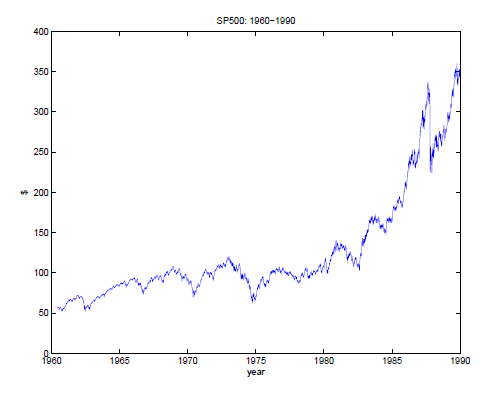
\includegraphics[width=100mm, height=70mm]{pics/sp500.png}

\end{frame}

\begin{frame}
\frametitle{Example: S\&P 500 stock}

Let $X_t$ denote the closing price of S\&P 500 stocks at the end of each month. We want to forecast the closing price of the stock for future observations. \\

\vspace{5mm}

\textbf{Question:} Should we regress $X_t$ against the time $t$ for our forecasts?

\end{frame}

\begin{frame}
\frametitle{Terminology}

\begin{itemize}

\item A \textbf{stochastic process} is a collection of random variables $X_t$ indexed by a set $T$, i.e. $t \in T$.


\item If $T$ consists of real numbers (or a subset), the process is called a \textbf{continuous time} stochastic process.

\item If $T$ is restricted to integers (or a subset), the process is called a \textbf{discrete time} stochastic process.

\item These processes may take on values which are real or restricted to integers and are called \textbf{continuous state space} or \textbf{discrete state space} respectively. 

\end{itemize}

\textbf{Question:} In the S\&P stock example, $X_t$ is a \textbf{discrete} time, \textbf{continuous} state space stochastic process.

\end{frame}

\begin{frame}
\frametitle{Terminology}

\begin{itemize}

\item Time series analysis is generally restricted to discrete time, continuous state space stochastic processes.

\item Continuous time, continuous state space stochastic processes are generally covered in a class for stochastic processes.

\end{itemize}

\end{frame}

\begin{frame}
\frametitle{Introduction to Time Series}

Time Series are data collected in a sequence.  They are usually evenly spaced and because of the sequential nature are statistically \textbf{dependent} observations.

\end{frame}

\begin{frame}
\frametitle{Introduction to Time Series}

In a regression setting, an assumption for data is that the observations are  \textbf{independent and identically distributed (iid),} i.e. the outcome at one point in the sequence does not effect the outcome at another point in the sequence.  The nature of our observations then will be a sequence of (typically real) numbers $x_1, \cdots,x_n$ where the index represents some type of ordering. Unlike iid sequences, order matters in time series.

\end{frame}

\begin{frame}
\frametitle{Introduction to Time Series}

\textbf{Question:} What are some consequences of using regression analysis on time series data?

\end{frame}





\section{Features of Time Series}
\frame{\tableofcontents[currentsection]}



\begin{frame}
\frametitle{Features}

Some of the features of time series data we look out for are:

\begin{itemize}
\item Trend.
\item Periodicity / Seasonality.
\item Is the mean changing over time?
\item Is the variation changing over time?
\item Are there abrupt changes?
\item Are there outliers?
\end{itemize}

Time series plots will be an important tool.

\end{frame}

\begin{frame}
\frametitle{Example: Monthly Sales at Souvenir Shop}

\begin{figure} \caption{Monthly sales for a souvenir shop at a beach resort town in Queensland, Australia, Jan 1987-Dec 1993.}
\begin{center}
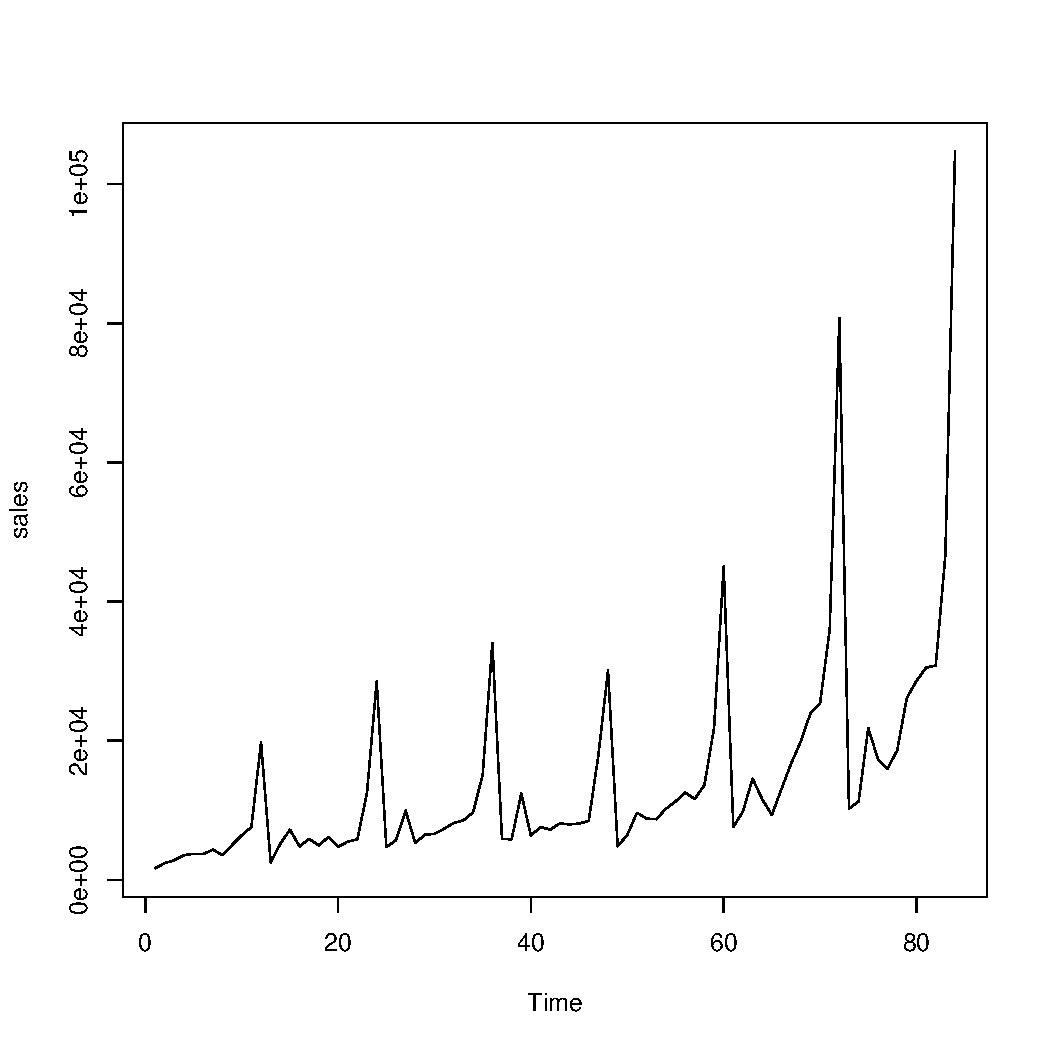
\includegraphics[width=100mm, height=60mm]{pics/shop.pdf}
\end{center}
\label{queensland}
\end{figure}

\end{frame}

\begin{frame}
\frametitle{Example: Monthly Sales at Souvenir Shop}

Regress sales on time index.

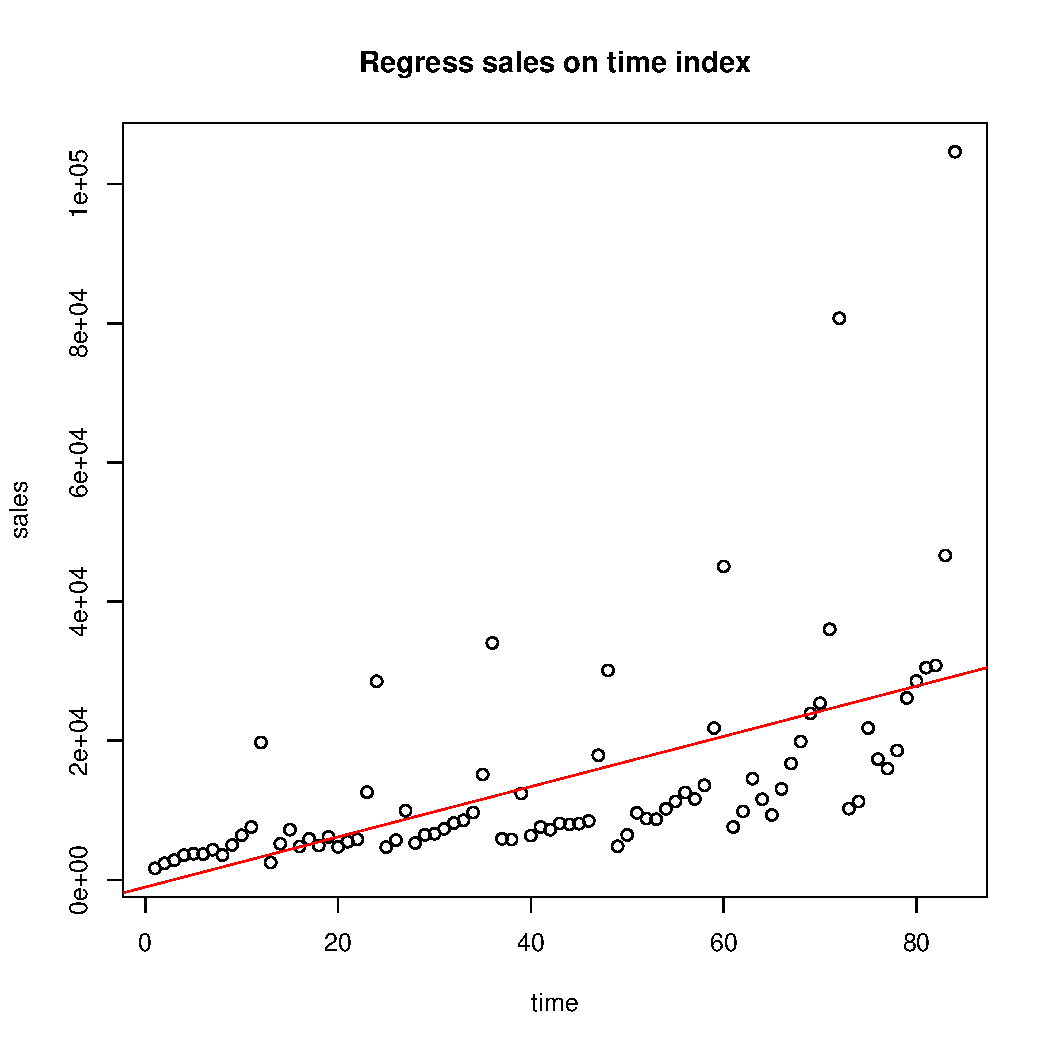
\includegraphics[width=100mm, height=50mm]{pics/regress.pdf}

Appears to be increasing trend.
\end{frame}

\begin{frame}
\frametitle{Example: Monthly Sales at Souvenir Shop}

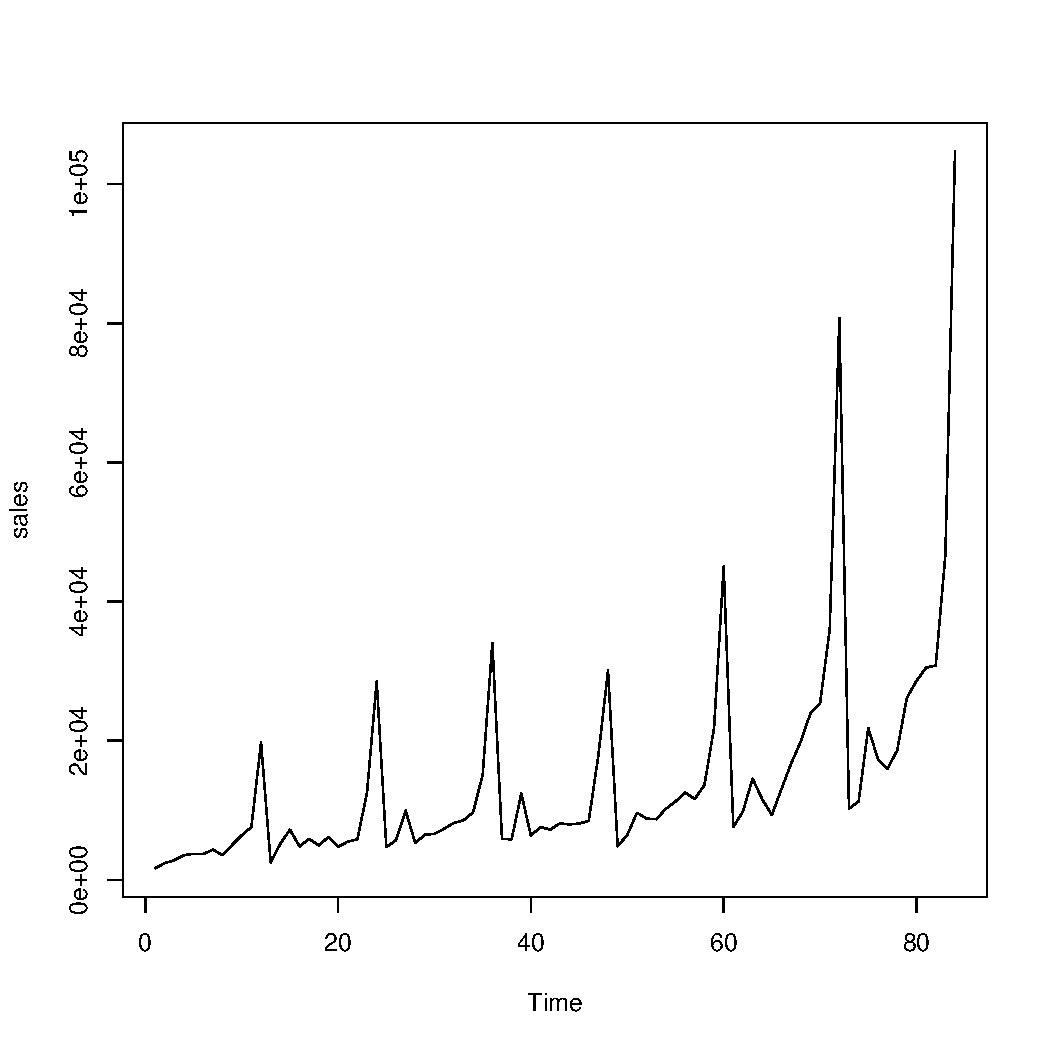
\includegraphics[width=100mm, height=60mm]{pics/shop.pdf}

Notice peaks at every 12 time period interval. Suggests presence of seasonality.

\end{frame}

%\begin{frame}
%\frametitle{Objectives of Time Series}
%\begin{enumerate}
%\item Description: Increasing sales with seasonality
%\item Interpretation: We need seasonal adjustment.
%\item Prediction: Predict sales.
%\item Control: Impact of policies on tourism.
%\item Hypothesis testing: Is trend/seasonality significant or due to chance.
%\item Simulation: Estimate probability of sales.
%\end{enumerate}
%\end{frame}

\section{Time Domain Vs Frequency Domain}
\frame{\tableofcontents[currentsection]}

\begin{frame}
\frametitle{Two Approaches to Time Series}
There are two primary approaches to time series.  One is the \textbf{time domain} approach.  This approach focuses on the rules for a time series to move forward. For example, how do yesterday's and today's observations affect tomorrow's observation?
\end{frame}

\begin{frame}
\frametitle{Two Approaches to Time Series}
The other approach is the \textbf{frequency domain} approach.  This approach tries to understand how differing oscillations can contribute to current observations. For example, taking hourly temperatures in Charlottesville, VA. There will be a very clear 24 hour oscillation.  There will be another clear 8,760 hour oscillation. The current temperature is a sum of these two sinusoids (plus a lot of noise and fluctuation).
\end{frame}

\section{A Few More Examples}
\frame{\tableofcontents[currentsection]}

\begin{frame}
\frametitle{Summer Temperature in Munich}

The next example is a series that involves the average summer temperature for each year in Munich from 1781 to 1988.
\end{frame}

\begin{frame}
\frametitle{Summer Temperature in Munich}

\begin{figure} \caption{Average Summer Temperature, Munich 1781-1988.}
\begin{center}
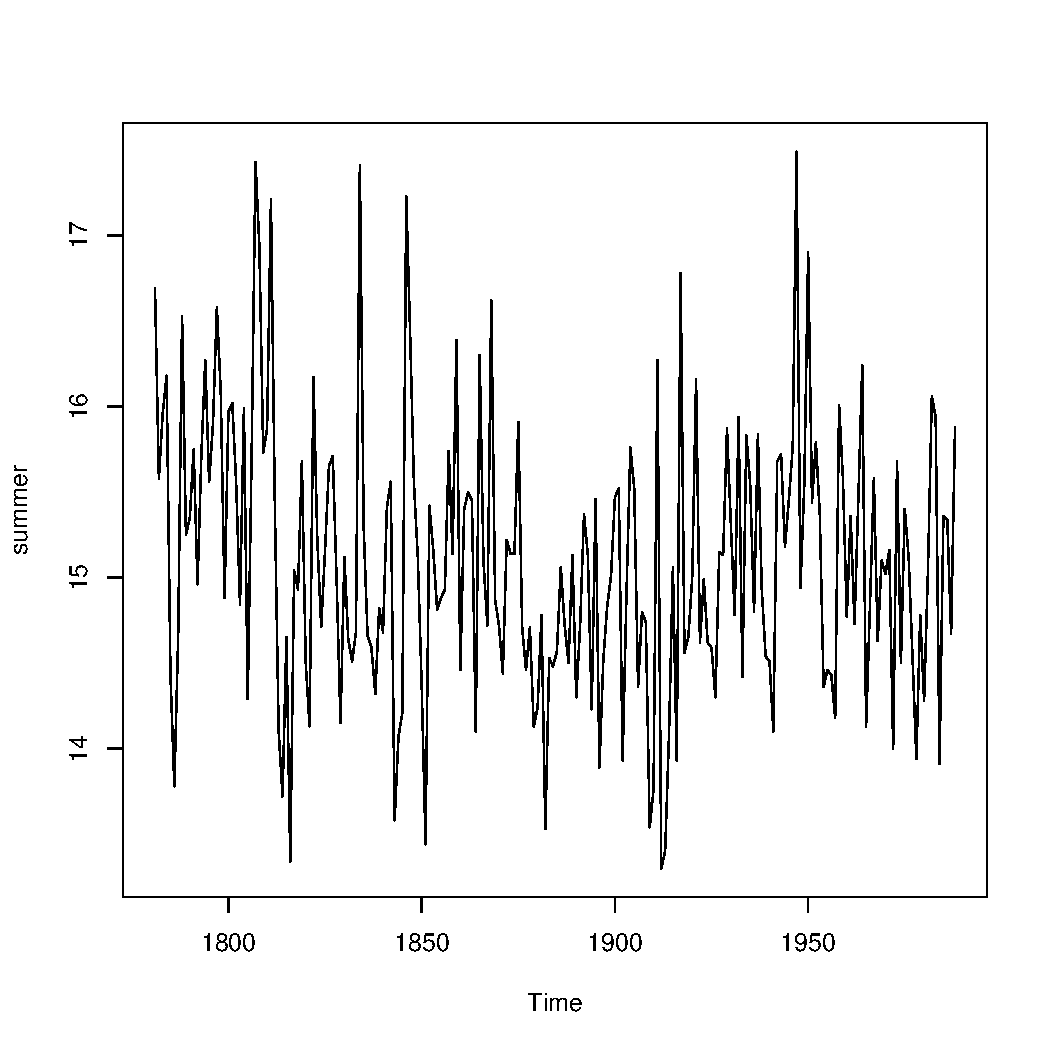
\includegraphics[width=100mm, height=60mm]{pics/summer.pdf}
\end{center}
\label{summer}
\end{figure}

\end{frame}

\begin{frame}
\frametitle{Summer Temperature in Munich}

The level of variance seems to be changing.  There seems to be a very mild sinusoidal trend.  It is usually not trivial to detect long range weather/climate trends at one location.
\end{frame}

\begin{frame}
\frametitle{Summer Temperature in Munich}
One way to assess independence is through \textbf{correlation}.  Independent random variables (RVs) are uncorrelated, but uncorrelated RVs may or may not be independent.  Mostly we'll be dealing with normal RVs in which case we won't have to worry about this. An autocorrelation plot is a tool which can aid us in assessing correlation

\end{frame}

\begin{frame}
\frametitle{Summer Temperature in Munich}

\begin{figure} \caption{ACF for summer data.}
\begin{center}
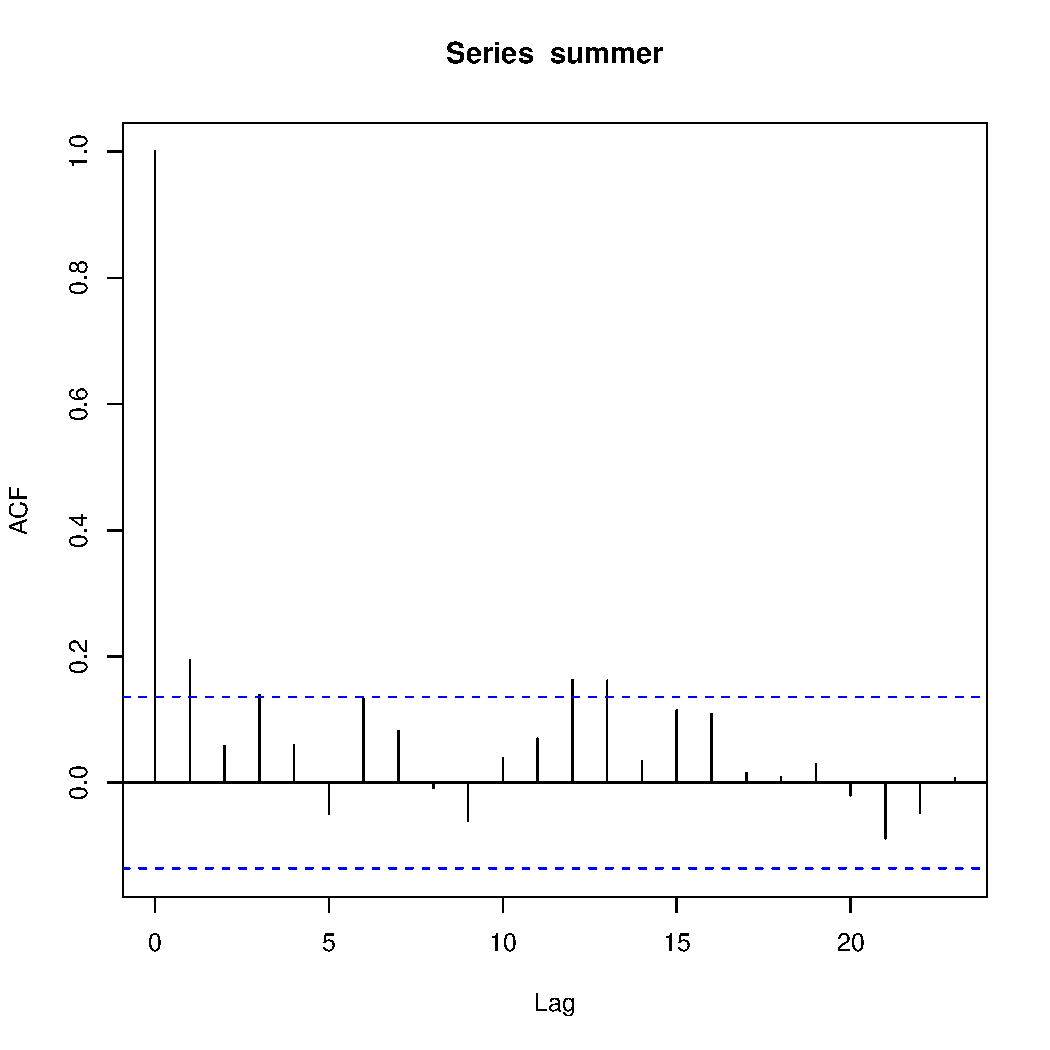
\includegraphics[width=100mm, height=60mm]{pics/summeracf.pdf}
\end{center}
\end{figure}

\end{frame}

\begin{frame}
\frametitle{Average Monthly Temperature in Dubuque, IA}

Another temperature time series is the average monthly temperature in Dubuque, IA. This is highly \textbf{periodic}. Later we'll talk about taking seasonal effects into account. We'll also discuss decomposing variation into Fourier components.
\end{frame}

\begin{frame}
\frametitle{Average Monthly Temperature in Dubuque, IA}

\begin{figure} \caption{Average monthly temperature: Dubuque, IA.}
\begin{center}
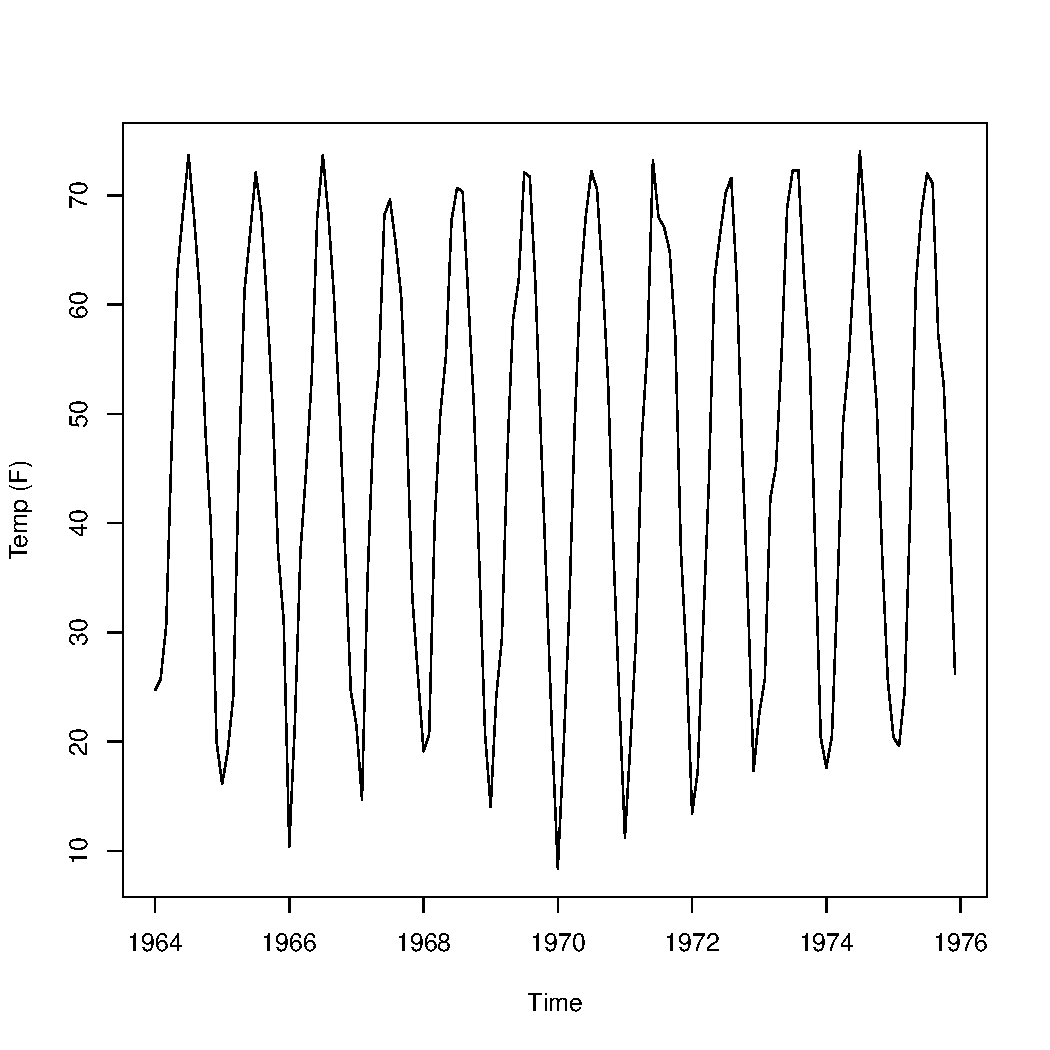
\includegraphics[width=100mm, height=60mm]{pics/dubuque.pdf}
\end{center}
\end{figure}

\end{frame}

\begin{frame}
\frametitle{Marriages in the Church of England}

There was a data set made famous by Yule concerning the number of marriages in the Church of England as a percentage of all marriages.  It appears as a somewhat negative linear trend. If we perform a linear regression, then the residuals are correlated.  We may want to tackle trends in a slightly different way to deal with the dependency.

\end{frame}

\begin{frame}
\frametitle{Marriages in the Church of England}

\begin{figure} \caption{Percent of Marriages in Church of England.}
\begin{center}
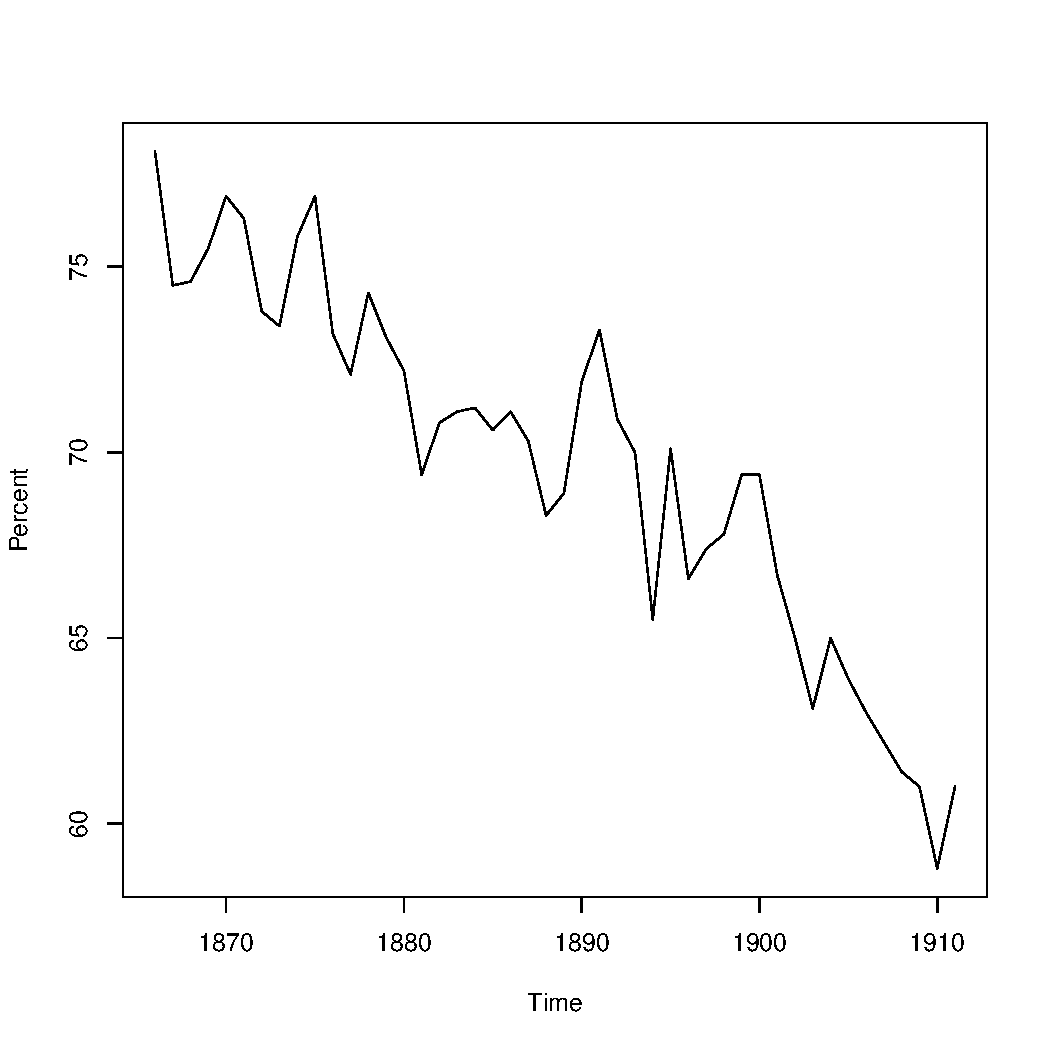
\includegraphics[width=100mm, height=60mm]{pics/marriage.pdf}
\end{center}
\end{figure}

\end{frame}

\begin{frame}
\frametitle{Marriages in the Church of England}

\begin{figure} \caption{ACF of residuals for marriage data.}
\begin{center}
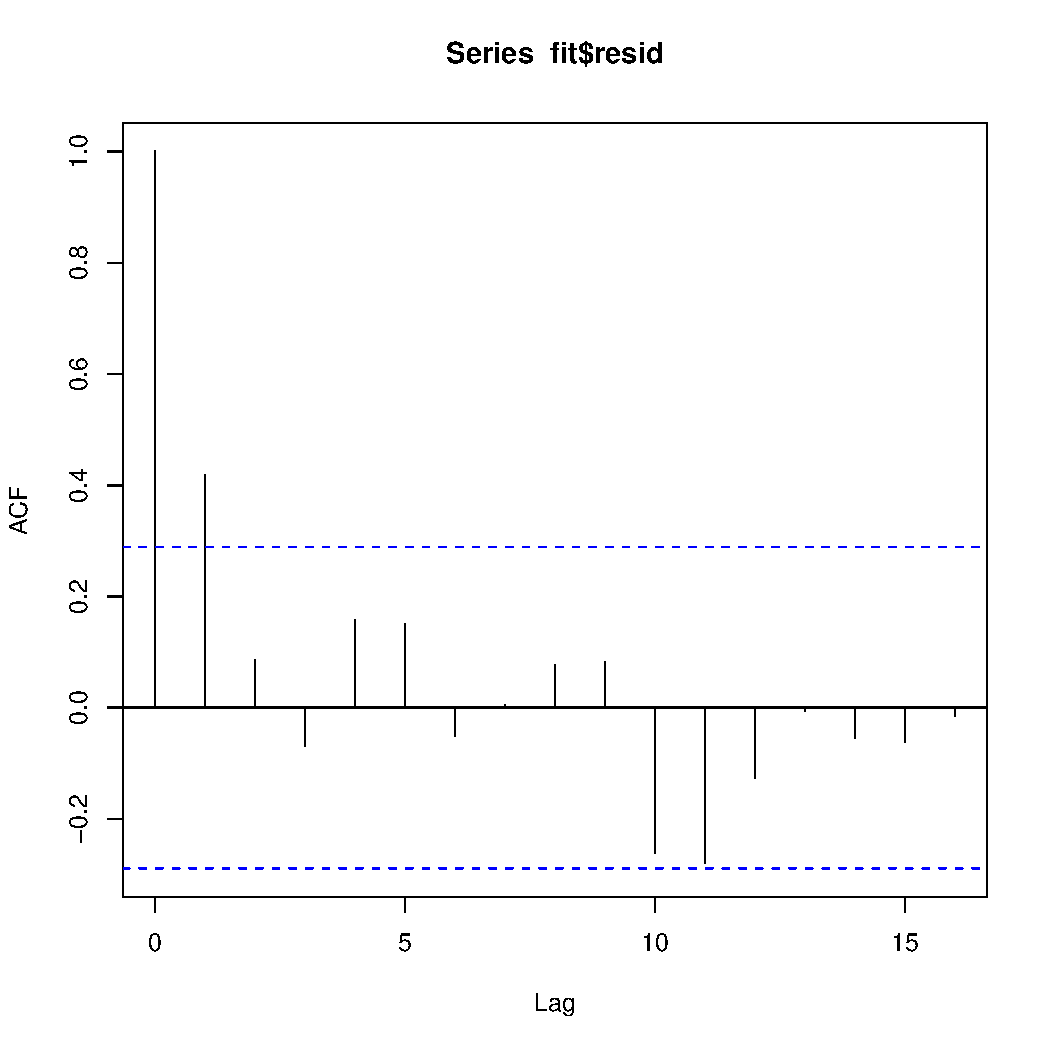
\includegraphics[width=100mm, height=60mm]{pics/marriageacf.pdf}
\end{center}
\end{figure}

\end{frame}

\begin{frame}
\frametitle{IBM Stock Prices}

In another data set with a clear trend, we look at the closing stock price for IBM stock from Jan 1980 to Oct 1992.  A common transformation for stock price is to look at returns $diff(log(x_n))$. The resulting series looks fairly \textbf{stationary} except for a huge shock. Different transformations get us data that's easier to analyze.

\end{frame}

\begin{frame}
\frametitle{IBM Stock Prices}

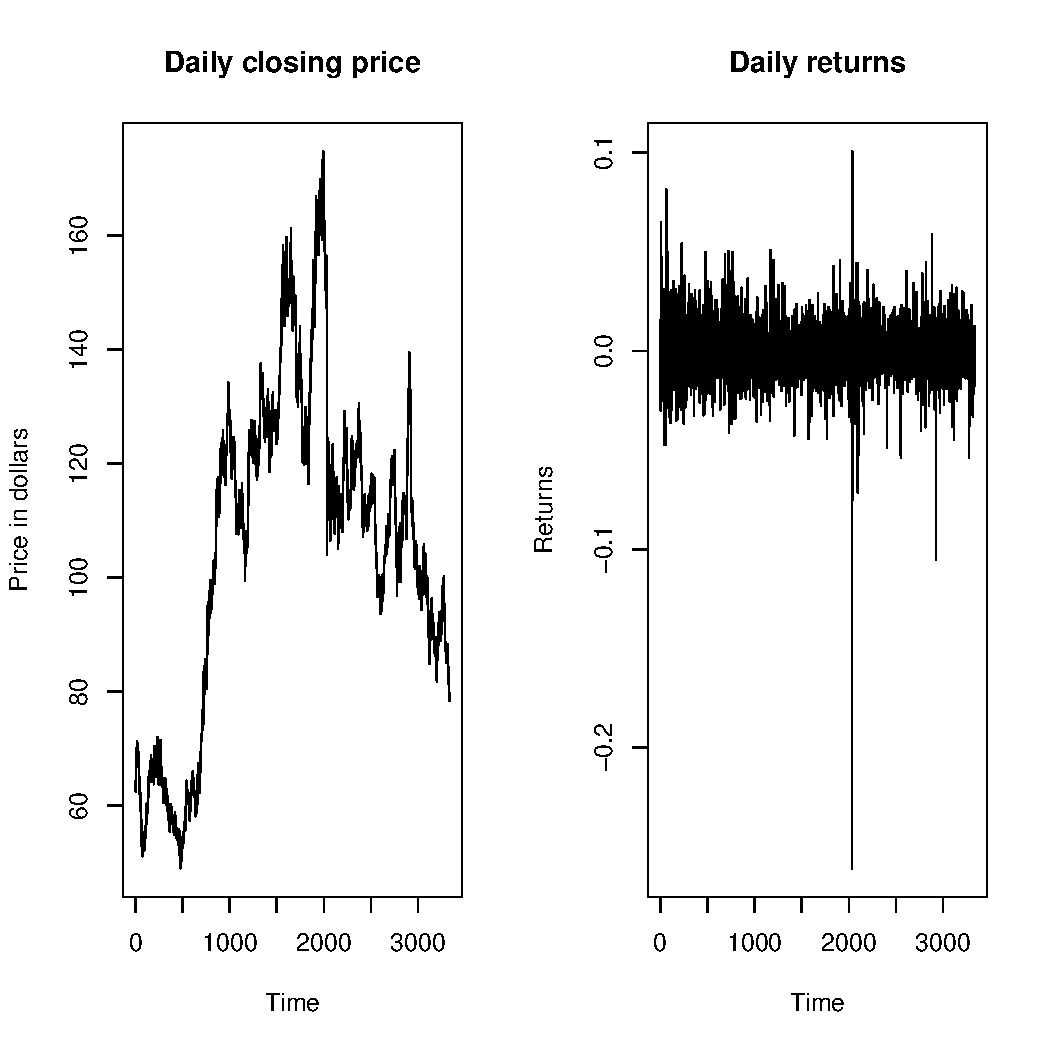
\includegraphics[width=100mm, height=60mm]{pics/ibm.pdf}

\end{frame}

\end{document} 